%\documentclass[iop]{emulateapj-rtx4}
% \shortauthors{French $\&$ Wakker}
%
%\usepackage{graphicx}
%\usepackage{subfigure}
%\usepackage{hyperref}
%\usepackage{amsmath}


%%%%%%%%%%
\documentclass[twocolumn,tighten]{aastex62}
%\documentclass{aastex6}
%\usepackage{emulateapj-rtx4}
%\usepackage{emulateapj}

 \shortauthors{French $\&$ Wakker}
\usepackage{graphicx}
\usepackage{subfigure}
\usepackage{amsmath}

%\usepackage{dblfloatfix}

%\usepackage{longtable}
%\usepackage{deluxetable}


\newcommand{\kms}{$\rm km\, s^{-1}$}
\newcommand{\HI}{\mbox{H\,{\sc i}} }

%\newcommand{\HI}{H\,{\sc i}}


\newcommand{\I}{\,{\sc i}}
\newcommand{\II}{\,{\sc ii}}
\newcommand{\III}{\,{\sc iii}}
\newcommand{\IV}{\,{\sc iv}}
\newcommand{\V}{\,{\sc v}}
\newcommand{\VI}{\,{\sc vi}}


\graphicspath{{figures//}}

\begin{document}

%\title{The environmental dependence of low-$z$ Ly$\alpha$ absorption}
\title{THE CIRCUMGALACTIC MEDIUM OF NEARBY GALAXIES: INTRODUCTION}


%Do Ly$\alpha$ absorbers co-rotate with galaxies?}

\author{David M. French, Bart P. Wakker}

\affil{Department of Astronomy, University of Wisconsin, Madison, WI 53706, USA}

\begin{abstract}


\end{abstract}


\keywords{galaxies:intergalactic medium, galaxies:evolution, galaxies:halos, quasars: absorption lines}


\section{INTRODUCTION}





%\begin{figure}[ht!]
%        \centering
%        \vspace{0pt}
%        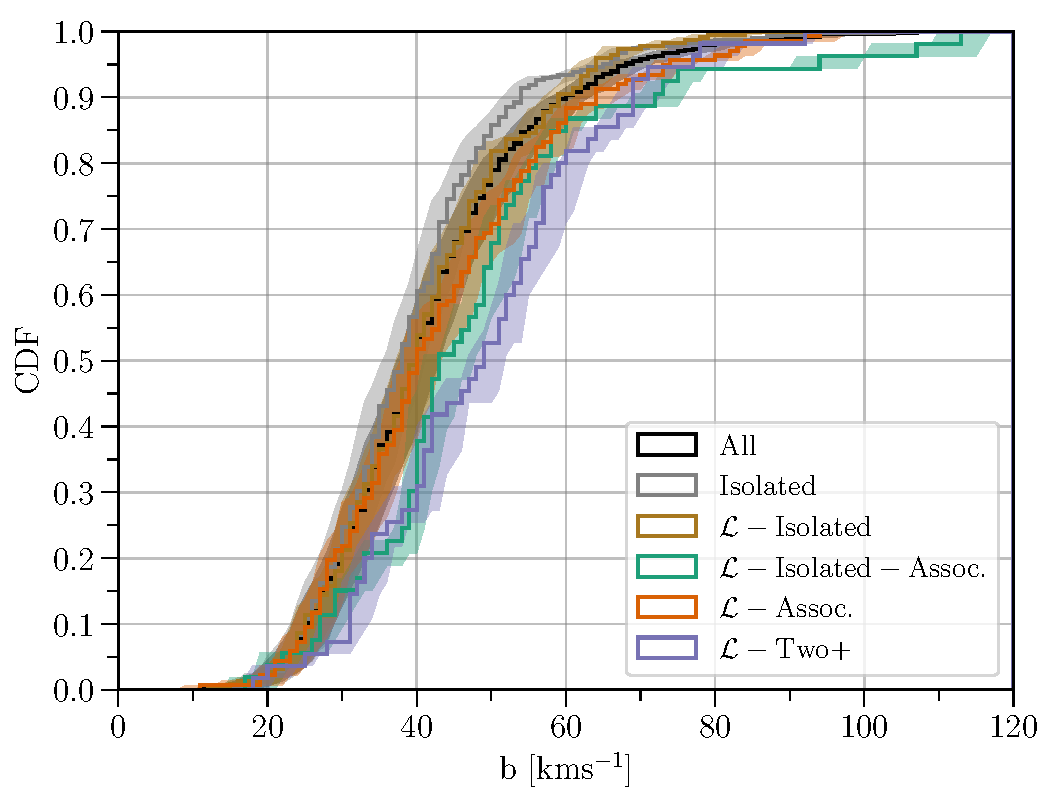
\includegraphics[width=0.49\textwidth]{hist(b)_all6_bins1_EWcut50-10000_errTrue_dataset.pdf}
%        \caption{\small{The Doppler $b$-parameter ($b$) cumulative distribution function for each subset of our Ly$\alpha$ absorber sample. From the top-left corner to the bottom-right the curves are the fully isolated absorbers (grey), the absorbers isolated enough from any galaxy to not be likelihood-matched (brown), the full distribution (black), the absorbers likelihood-matched to a single, non-isolated galaxy (orange), the absorbers matched to a single, isolated galaxy (green), and the absorbers likelihood-matched with two or more galaxies (purple). The shaded region around each curve gives the $b$-parameter measurement errors. Only $\rm EW \ge 50~m\AA$ absorbers are included to mitigate any bias due to the detection limit of lower-SN targets.}}
%        \vspace{5pt}
%        \label{cdf_b}
%\end{figure}

\section{Outline of Thesis}

In the chapters that follow I 

2. In Chapter 2 I present our new nearby galaxy catalog, which we will later use to study the environment of $\rm Ly\alpha$ absorption lines detected in COS spectra. This catalog has been compiled entirely from the published data made available by the NASA Extragalactic Database (NED), the NASA/IPAC Infrared Science Archive (IRSA), and the \cite{tully2015} 2MASS galaxy group catalog. We discuss our data retrieval methods, the numerous ways we have attempted to homogenize galaxy data, and also discuss the completeness of the catalog. 

3. In Chapter 3 I present our pilot study, \cite{french2017}. This study contained a sample of 33 COS sightlines toward background QSOs, chosen for their proximity to large ($D \ge 25$ kpc) galaxies. We introduce a new method for algorithmically matching absorbers to nearby galaxies

4. In Chapter 4 I present our study of the kinematics of $\rm Ly\alpha$ absorption in comparison to the disk rotation of nearby galaxies. 

\acknowledgements

D. M. F. thanks \textbf{A BUNCH OF PEOPLE}.This research has made use of the NASA/IPAC Extragalactic Database (NED) which is operated by the Jet Propulsion Laboratory, California Institute of Technology, under contract with the National Aeronautics and Space Administration. Based on observations with the NASA/ESA \textit{Hubble Space Telescope}, obtained at the Space Telescope Science Institute (STScI), which is operated by the Association of Universities for Research in Astronomy, Inc., under NASA contract NAS 5-26555. \textbf{SALT ACKNOWLEDGEMENT}. Spectra were retrieved from the Barbara A. Mikulski Archive for Space Telescopes (MAST) at STScI. Over the course of this study, D.M.F. and B.P.W. were supported by grant XXXX

%AST-1108913, awarded by the US National Science Foundation, and by NASA grants \textit{HST}-AR-12842.01-A, \textit{HST}-AR-13893.01-A, and \textit{HST}-GO-14240 (STScI). 

\facility{HST (COS), SALT (RSS)}
\clearpage

%\nocite{*}
%\bibliography{rotation_bib}
%\bibliography{/Users/frenchd/Research/bib}{}
\bibliography{/Users/frenchd/Research/inclination/git_inclination/bib}{}
\bibliographystyle{apj}

\clearpage

\appendix

\end{document}
